% !TeX root = ../main.tex

\chapter{个人贡献}

在此次大作业中,我负责使用 Python 语言实现算法 (\ref{Algorithm:RMFA}) 和算法 (\ref{Algorithm:DFAS}) 的原型并为组内其他成员提供基本的绘图框架。在进行对上述两个算法的实现中,我发现精度对算法正确性有着不小的影响,不确定的精度会影响断点的位置,使得断点或在上、或在下,如图 (\ref{Error}) 所示。

\begin{figure}[htb]
    \centering
    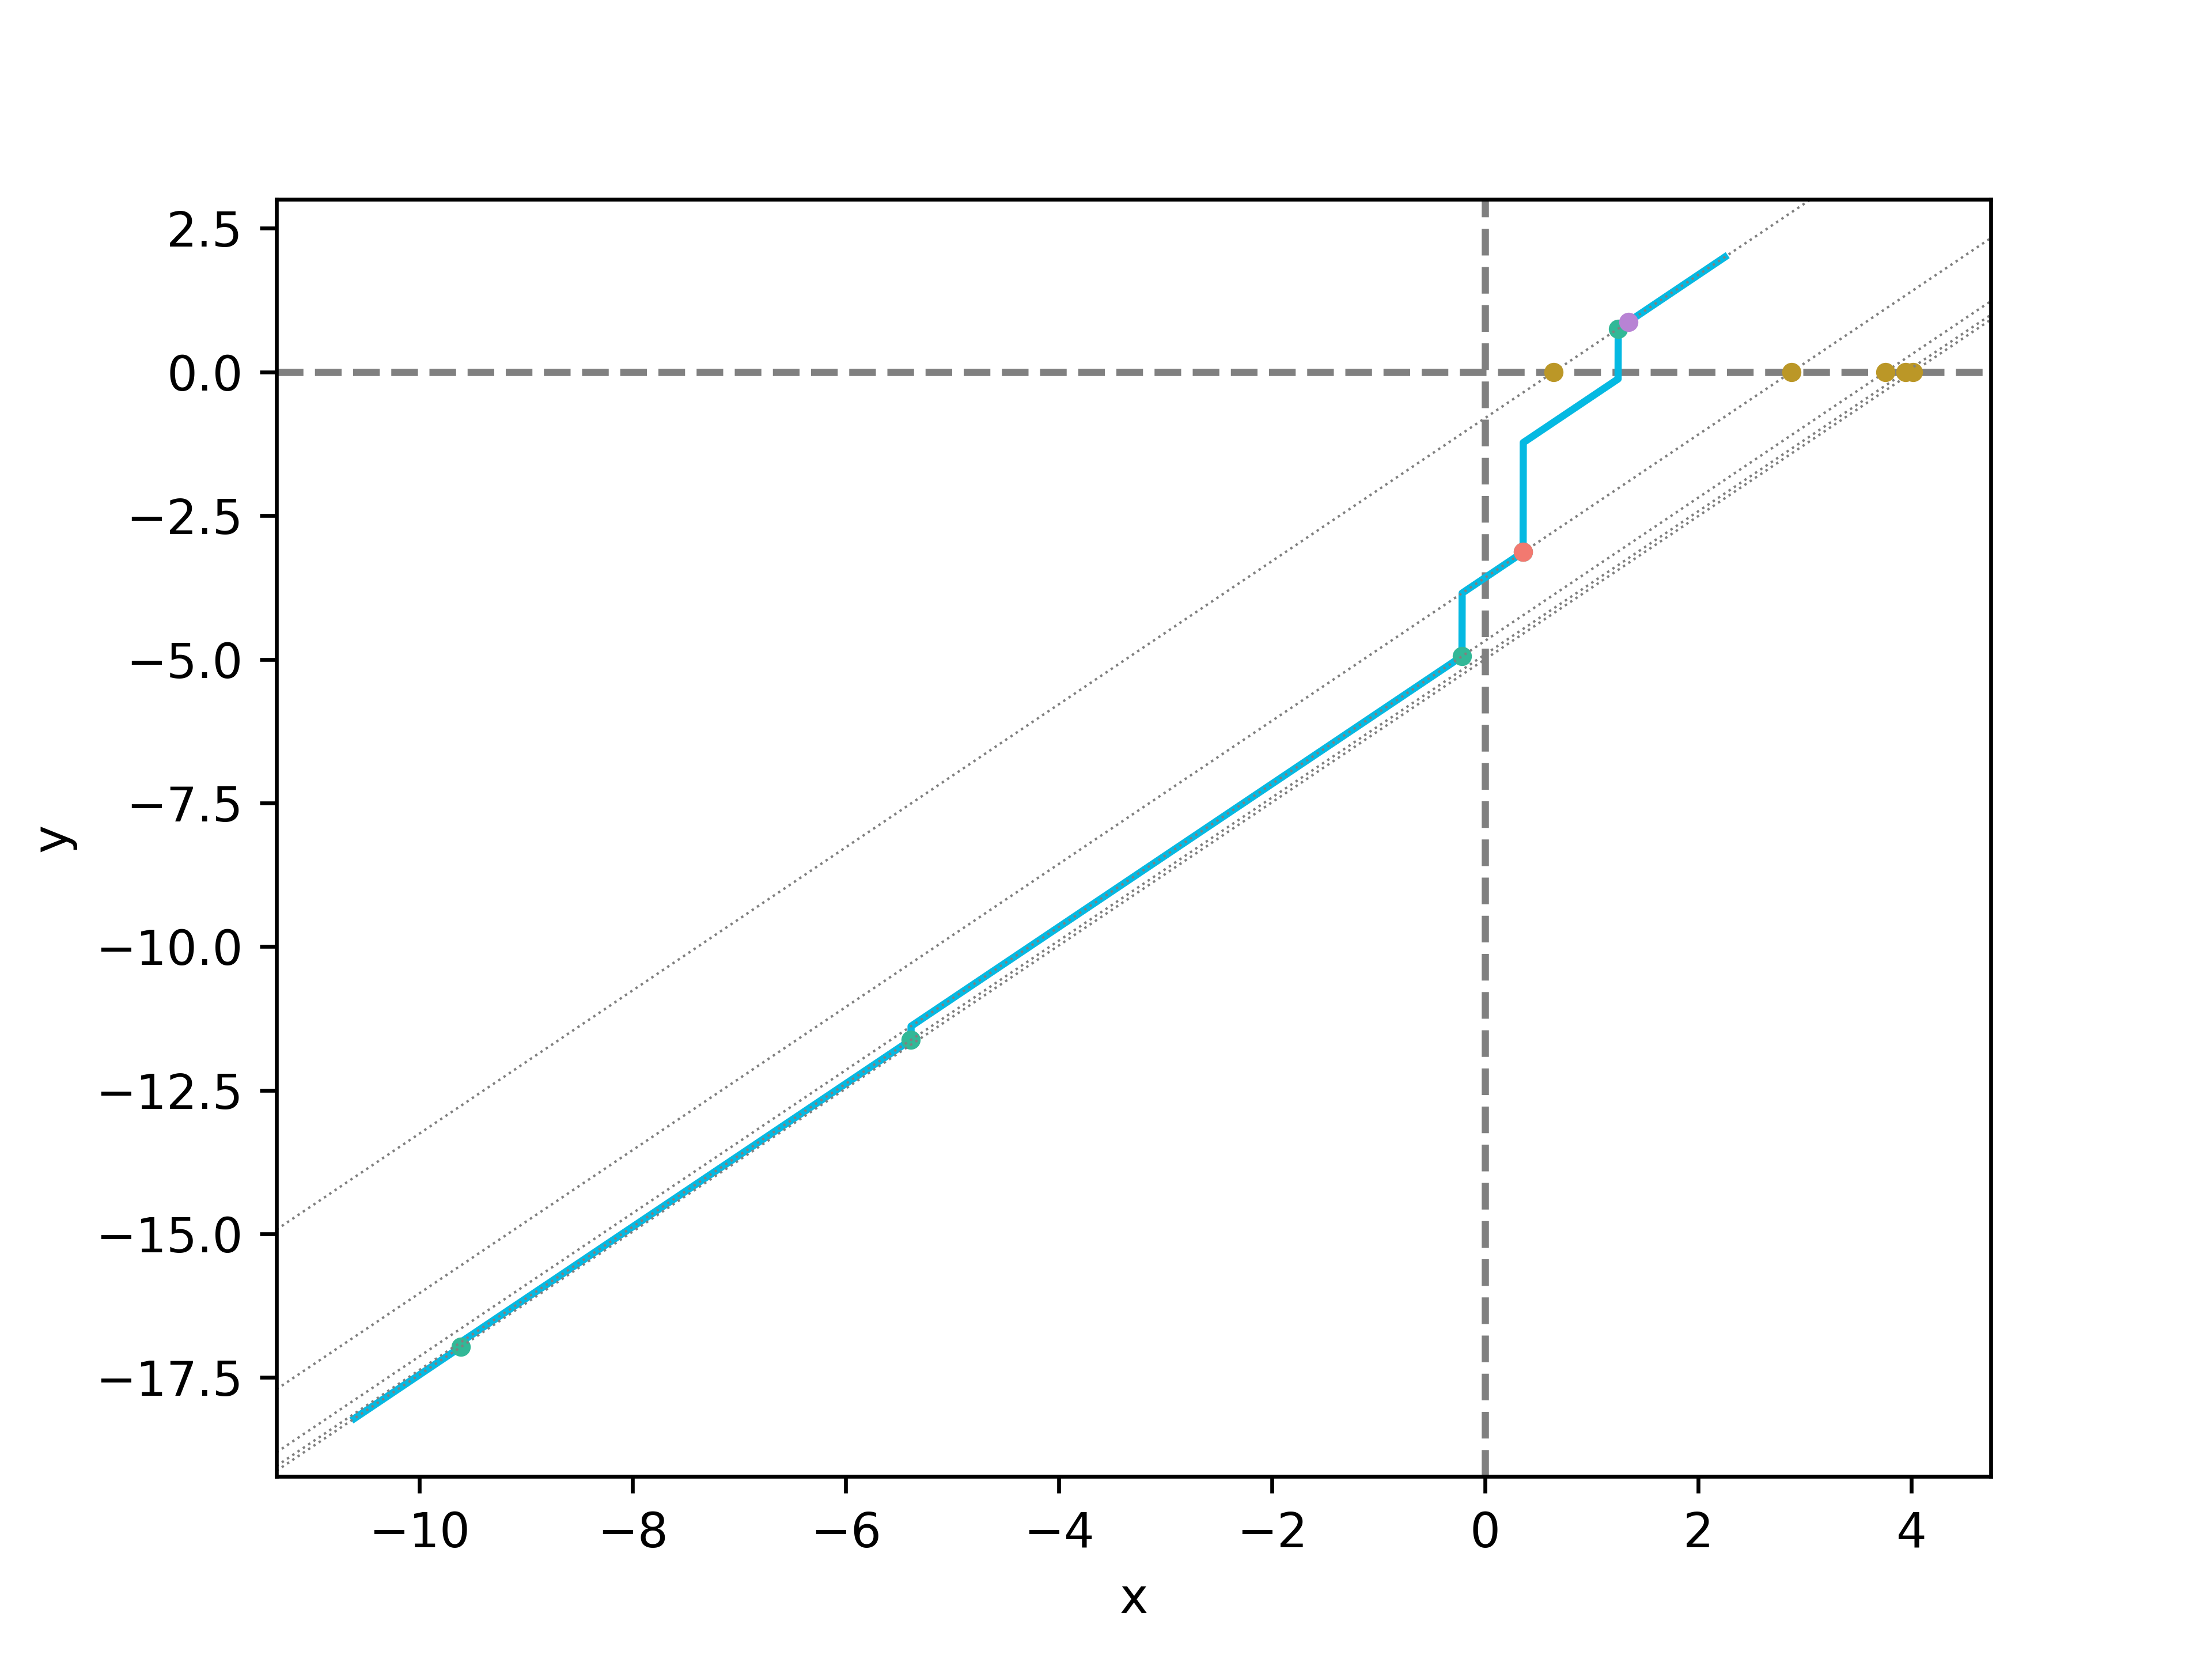
\includegraphics[width=0.5\textwidth]{figures/Error.png}
    \caption{错误的次梯度函数图像}
    \label{Error}
\end{figure}

可以看到,在图 (\ref{Error}) 中,断点(绿色点)的位置并非确定的在上方或下方,而是或上或下。两个算法所求的解也均不正确,算法 (\ref{Algorithm:RMFA}) 所求的解(紫色点)偏上,算法 (\ref{Algorithm:DFAS}) 所求的解(红色点)偏下。

为了解决这个问题,首先要固定断点的位置。要固定断点的位置,一种简单的方法是:令精度为 $10^{-8}$,对每个断点向 $x$ 轴负半轴偏移 $10^{-8}$。此时,所有的断点均被固定于下方,如图 (\ref{SubGradient}) 和图 (\ref{Answer}) 所示。在固定断点的位置后,再次使用算法 (\ref{Algorithm:RMFA}) 和算法 (\ref{Algorithm:DFAS}) 进行求解便可以得出正确的结果,具体的实现请参考相关源代码。

Python 语言实现的算法原型代码已经上传至 \href{https://github.com/xqm32/unix-report-python}{https://github.com/xqm32/unix-report-python},仓库中还包含了组内其他成员编写的性能对比、图像绘制的代码。